\section{Conceptual Framework}
\label{sec:concept}

\begin{figure}[H]
\centering
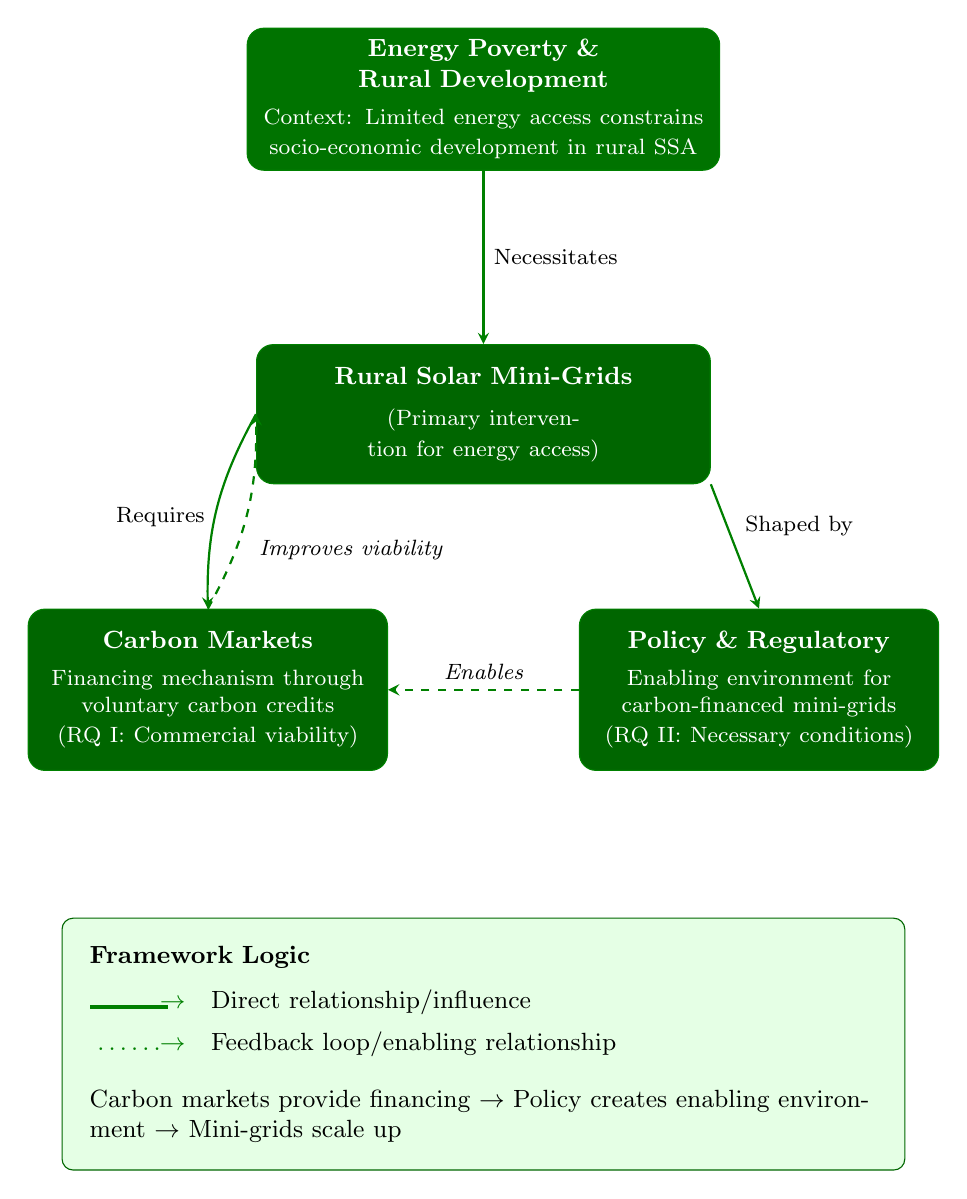
\begin{tikzpicture}[
  every node/.style={font=\small},
  topbox/.style={
    rectangle, rounded corners=6pt,
    draw=green!50!black, fill=green!45!black,
    text=white, text width=6cm, align=center,
    minimum height=1.4cm, inner xsep=0pt, inner ysep=4pt
  },
  mainbox/.style={
    rectangle, rounded corners=6pt,
    draw=green!50!black, fill=green!40!black,
    text=white, text width=5.2cm, align=center,
    minimum height=1.4cm, inner sep=8pt
  },
  sidebox/.style={
    rectangle, rounded corners=6pt,
    draw=green!50!black, fill=green!40!black,
    text=white, text width=4.0cm, align=center,
    minimum height=2.0cm, inner sep=8pt
  },
  legendbox/.style={
    rectangle, rounded corners=4pt,
    draw=green!40!black, fill=green!10,
    text=black, text width=10cm, align=left,
    inner sep=10pt
  },
  solidarrow/.style={
    ->, >=stealth, thick, green!50!black
  },
  dasharrow/.style={
    ->, >=stealth, thick, dashed, green!50!black
  },
]

% --- Nodes ---
\node[topbox] (poverty) at (0, 7.5)
  {\textbf{Energy Poverty \& Rural Development}\\[4pt]
   \footnotesize Context: Limited energy access constrains\\socio-economic development in rural SSA};

\node[mainbox] (minigrids) at (0, 3.5)
  {\textbf{Rural Solar Mini-Grids}\\[4pt]
   \footnotesize (Primary intervention for energy access)};

\node[sidebox] (carbon) at (-3.5, 0)
  {\textbf{Carbon Markets}\\[4pt]
   \footnotesize Financing mechanism through voluntary carbon credits\\(RQ I: Commercial viability)};

\node[sidebox] (policy) at (3.5, 0)
  {\textbf{Policy \& Regulatory}\\[4pt]
   \footnotesize Enabling environment for carbon-financed mini-grids\\(RQ II: Necessary conditions)};

% --- Solid arrows ---
% Necessitates: poverty -> minigrids
\draw[solidarrow] (poverty.south) -- node[right, text=black]{\footnotesize Necessitates} (minigrids.north);

% Shaped by: minigrids -> policy
\draw[solidarrow] (minigrids.south east) -- node[above right, text=black]{\footnotesize Shaped by} (policy.north);

% Requires: minigrids -> carbon (solid, outer arc bowing left/west)
\draw[solidarrow] (minigrids.west)
  to[bend right=15]
  node[left, pos=0.55, text=black, font=\footnotesize]{Requires}
  (carbon.north);

% --- Dashed arrows ---
% Improves viability: carbon -> minigrids (dashed, inner arc bowing right/east)
\draw[dasharrow] (carbon.north)
  to[bend right=15]
  node[right, pos=0.55, yshift=-16pt, text=black, font=\footnotesize\itshape]{Improves viability}
  (minigrids.west);

% Enables: policy -> carbon
\draw[dasharrow] (policy.west)
  -- node[above, text=black, font=\footnotesize\itshape]{Enables}
  (carbon.east);

% --- Legend ---
\node[legendbox] at (0, -4.5) {
  \textbf{Framework Logic}\\[6pt]
  \begin{tabular}{@{}l@{\quad}l@{}}
    {\color{green!50!black}\rule{1cm}{1.5pt}$\!\!\rightarrow$} & Direct relationship/influence \\[4pt]
    {\color{green!50!black}\makebox[1cm]{\dotfill}$\!\!\rightarrow$} & Feedback loop/enabling relationship \\[6pt]
  \end{tabular}\\[4pt]
  Carbon markets provide financing $\rightarrow$ Policy creates enabling environment $\rightarrow$ Mini-grids scale up
};

\end{tikzpicture}
\caption{Conceptual framework linking energy poverty, rural solar mini-grids, carbon markets, and policy.}
\label{fig:concept}
\end{figure}

The conceptual framework examines how carbon markets can support rural solar mini-grid deployment in SSA through interconnected components.

\begin{enumerate}
	\item \textbf{Carbon markets} as a financing mechanism, where voluntary credits can improve commercial viability but face uncertainties around transaction costs and certification, host government authorization, and revenue leakage to intermediaries.~\cite{kreibich2021,michaelowa-evolution,ahonen-governance}
	\item \textbf{Policy, regulatory, financial and technical frameworks,} which shape enabling conditions but often lack integration between energy regulations and carbon mechanisms, particularly regarding Article 6 authorization requirements and carbon revenue treatment within tariff structures.~\cite{esmap2019,bhattacharyya2016,schneider-integrity}
\end{enumerate}

Feedback loops link these components: regulatory clarity facilitates carbon market participation, and carbon finance strengthens commercial viability, enabling larger-scale projects. The framework guides investigation of barriers and enabling conditions across both RQs, with particular attention to structural market failures that prevent aggregation mechanisms from emerging organically.
